\subsection{\label{sec:multigrid}Multigrid}
The implementation of the multigrid solver algorithm in LFRic has taken a
long time to develop for several reasons. Firstly, the new solver API,
which enables easy configuration of different solver algorithms and
pre-conditioners\footnote{Even nested solvers as currently deployed.},
uses advanced Fortran OO abstract types. This has caused most
compilers to have problems and significantly delayed the
implementation. Secondly, implementing multigrid itself required
several infrastructure changes. Multiple meshes, maps between these
meshes and support for intergrid kernels in the PSyKAl API and in
PSyclone. These have all been successfully implemented. Thirdly, when
the multigrid algorithm itself was implemented the solver had problems
converging.
This was ultimately resolved as an issue with the vertical
pre-conditioner and not multigrid itself. 

The multigrid algorithm implemented here is a four-level V-cycle of
the horizontal mesh, and used to pre-condition the Helmholtz or
pressure solver. In fact, the pre-conditioned pressure field is taken
as the ``solved'' outcome and no iterative, Krylov solver is applied
to the pressure system. The outer solver of the mixed system uses the
GCR algorithm. The algorithmic details are not discussed here, but a
Krylov sub-space solver performs several global sums per iteration. As
multiple solves per outer iteration are required, each itself of many
iterations there is a reduction of several thousand global sums per
time-step employing multigrid in ths manner.

Neither the change to the vertical pre-conditioner, nor the multigrid
solver are on the trunk. There is nothing to suggest that they require
significant alteration, but the process of getting them on trunk has
yet to be completed. Therefore results presented here for the
Multigrid performance should be regarded as preliminary.

\begin{table}
\centering
\caption{\label{tab:MG_data}Wall-clock time of execution of the whole code (WC), User
  code (U), Halo Exchange (HE) and Global Sum (GS) in seconds. T17483
  denotes the trunk at revision 17483, MG-B the CSAR branch,
  Krylov uses a Krylov solver and MG the multigrid pre-conditioner as
  the solver.
}
\begin{tabular}{r|rrrr}
version     & WC     & U      & HE     & GS \\\hline
T17483      & $5398$ & $1851$ & $1333$ & $1657$ \\
MG-B Krylov & $3387$ & $1087$ & $847$  & $1080$ \\
MG-B MG     & $1337$ & $504$  & $388$  & $199$ \\\hline
\end{tabular}
\end{table}

\begin{figure}[ht!]
\centering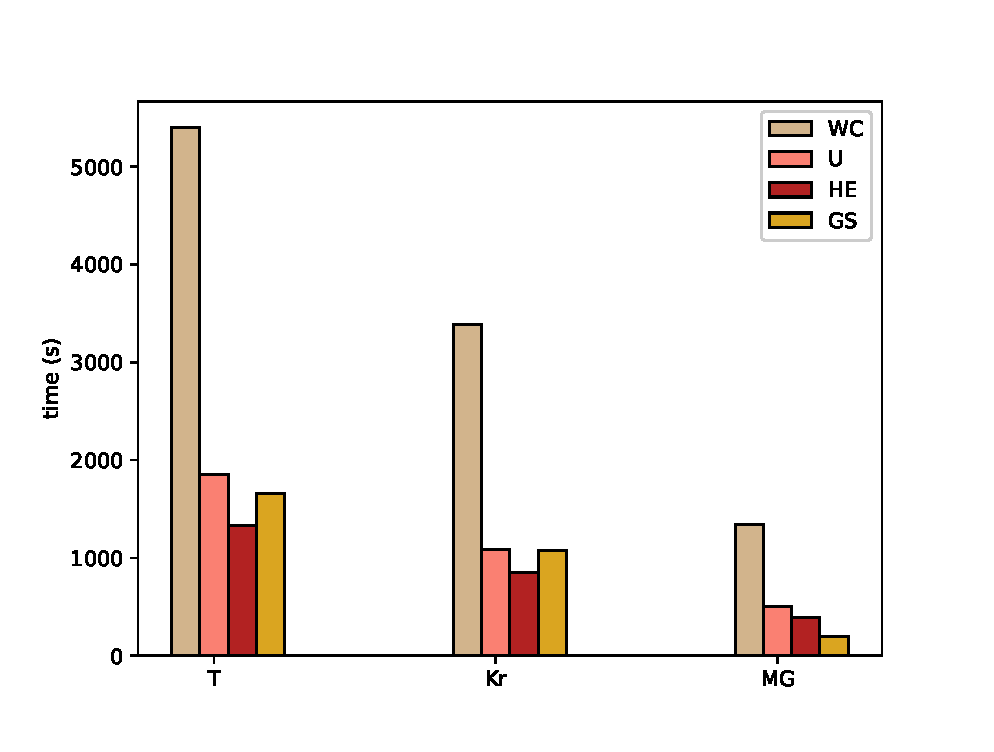
\includegraphics[width=1.0\linewidth]{figs/mg-improvement.eps}
\caption{\label{fig:mg}Wall-clock time for model components of
  Baroclinic Wave test. ``T'' denotes trunk at 17483, ``Kr'' denotes
  CSAR branch with the Krylov subspace solver and ``Mg'' denotes
  CSAR branch with the multigrid pre-conditioner as the solver.}
\end{figure} 

Displayed in Table~\ref{tab:MG_data} and shown in figure~\ref{fig:mg}
are the profiling data from CrayPAT for three different model versions
of the Baroclinic wave test on a $C1152$ mesh with a $120$s time-step
for $100$ time-steps. This corresponds to a roughly 9km
resolution. The models were run on $384$ nodes with $6$ MPI ranks per
node and $6$ Open MP threads per MPI rank.  The CSAR branch is \verb+r17264_CSAR19_gungho@17480+.